\chapter{C\# language}
The goal of this chapter is to introduce C\# programming language and .NET platform. The following part of the chapter will focus on NuGet package manager as it forms a building block for the upcoming text. Furthermore, ASP.NET Core framework's background will be described, accompanied by an introduction to Razor markup, which is tightly entangled with ASP.NET Core. Both the ASP.NET Core part and the Razor part will also present an overview of their usage with simple code examples.

\section{Language introduction}
C\# is a general-purpose programming language, under the management of Microsoft Corporation. It is a part of the developer platform called .NET. One of the main features of .NET is language interoperability, giving programmer opportunity to combine multiple languages and libraries in a single project. That is possible because of the same specification that all .NET components are build atop, called the Common Language Infrastructure (CLI) \citep{Ecma335}. The CLI has been standardized by ECMA International in ECMA-335 and approved as ISO/IEC 23271 \citep{Ecma335}. This document covers following 4 areas of interest: type system, metadata, the Common Language Specification (CLS) and the Virtual Execution System (VES) \citep{Ecma335}. 

At the time of writing, there are 8 major versions of C\# programming language released \citep{microsoft.docs}. When speaking of C\# we implicitly mean C\# version 8, as the latest officially released version.

\paragraph{Type system}
The question of types and their definitions is answered by the Common Type System (CTS) \citep{Ecma335}. In order to cover type systems of wide range of programming languages, the CTS defines large number of types and operations \citep{Ecma335}. 

\paragraph{Metadata}
\textit{"Metadata are used as a way to describe and reference the types defined by the CTS. For that purpose, they are stored in a way that is independent of any particular programming language"} \citep{Ecma335}.

\paragraph{Assemblies}
With language-unique compilers, each .NET project is compiled to the Common Intermediate Language (CIL), also known as managed code or simply IL \citep{Ecma335, ProCSharp}. Resulted compiled code is then saved as either a Dynamically Linked Library (DLL) or en Executable file (EXE) \citep{ProCSharp}. Basically, when the compiled code specifies the application's entry point, EXE file is generated, DLL file is generated otherwise \citep{ProCSharp}. Exception to this behaviour brought .NET Core, which makes it possible to generate DLL files for both, code with and without an entry point \citep{microsoft.docs}. Generated DLLs and EXEs together are called assemblies \citep{ProCSharp}.

\paragraph{The Common Language Specification}
The CLS specifies a subset of the CTS and a set of rules that publicly exported aspects of compiled assemblies shall follow in order to ensure language interoperability \citep{Ecma335}. Its aim is to provide developers with the same base types and usage conventions for each framework that adhere the CLS. \citep{Ecma335}

\paragraph{Virtual Execution System}
The VES is responsible for loading and running programs written for the CTS \citep{Ecma335}. It provides the services needed to execute managed code and data, using the metadata to connect separately generated modules together at runtime (late binding) \citep{Ecma335}. On runtime, platform-specific implementation of the VES performs just-in-time (JIT) compilation of the CIL code to the native code \citep{Ecma335}.

\paragraph{.NET Standard}
In addition to the CLI, .NET Standard was introduced as a way to establish greater uniformity in the .NET environment \citep{ProCSharp}. In contrary to the CLI, .NET Standard only specifies a set of .NET APIs that are intended to be available on all .NET implementations \citep{microsoft.docs}. Each version of major .NET implementation, such as .NET Core, .NET Framework or Mono, targets specific versions of .NET Standard \citep{microsoft.docs}. Each application can target a version of a specific .NET implementation or version of .NET Standard, making it possible to run on any .NET implementation which supports that version of the .NET Standard \citep{ProCSharp}.

\paragraph{}
The process of C\# application's deployment from compilation to execution is summed up in the following Figure.

\begin{figure}[h]
  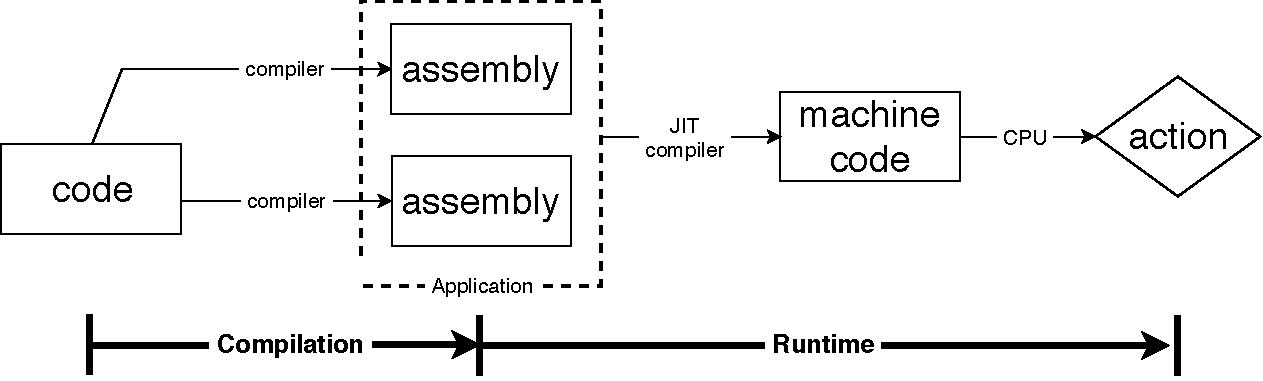
\includegraphics[width=\linewidth]{img/Csharp.pdf}
  \caption{C\# application's deployment}
  \label{fig:csharp_execution}
\end{figure}


\section{Language features}

\paragraph{Type system}
Types in C\# are divided into two main categories, value types and reference types. In contrary to value types, that directly hold their data, reference types hold only references to objects. There is also a type called \texttt{System.Object}. It is the base class of all types in C\#, meaning that every type in C\# can be converted to an object type (boxing) and vice versa (unboxing) \citep{microsoft.docs}. Because of that, the type system of C\# can be label as a Unified Type System. 

Slightly aside from this, stands the dynamic type. Its features are, in terms of boxing and unboxing, very close to those of base object type \citep{microsoft.docs}. The point where dynamic type differs from base object type is in the amount of information compiler has about the type, and in the way type is processed on runtime \citep{microsoft.docs}. An example illustrating both those differences is casting \citep{microsoft.docs}. Dynamic variables do not require any explicit type casting, fully relying on the programmers' knowledge of what he or she is doing \citep{microsoft.docs}. Main purpose of dynamic types is to allow interactions with dynamic objects, such as objects from other programming languages with type systems different than the one of C\# \citep{microsoft.docs}.

\paragraph{Variables}
In C\#, every variable has a type that determines what values can be stored in the variable \citep{microsoft.docs}. On compilation, C\# compiler validates whether each value stored in a variable is of the appropriate type and whether there are no operations with given variable, that are invalid for its type \citep{microsoft.docs}. In other words, C\# is type safe.

There is also requirement for each variable to be definitely assigned before C\# compiler allows for its value to be obtained \citep{microsoft.docs}. Microsoft documentation defines definitely assigned variable as follows: \textit{"At a given location in the executable code of a function member, a variable is said to be definitely assigned if the compiler can prove, by a particular static flow analysis, that the variable has been automatically initialized or has been the target of at least one assignment"} \citep{microsoft.docs}. 


\section{NuGet}
NuGet is Microsoft-supported mechanism for creating, sharing and consuming code under the .NET environment \citep{microsoft.docs}. For this purpose NuGet defines a \texttt{package}, single unit of compiled code, related resources and a descriptive manifest containing necessary information about both, the package and the code it holds \citep{microsoft.docs}. These packages are generally nothing more than a \texttt{.zip} archive of mentioned three groups of files with \texttt{.nupkg} extension \citep{microsoft.docs}. 

In order to allow other developers to download and use a package, when created, a package is usually published to some kind of a sharing service \citep{microsoft.docs}. Depending on desired accessibility level, it can be publicly accessible hosting service such as \texttt{nuget.org}, a cloud, a network or a local file system \citep{microsoft.docs}.

Prior to a package usage, one must first ensure that the package and its required version has been installed \citep{microsoft.docs}. Regardless the method used for the package installation, NuGet always merges \texttt{packageSources} from \texttt{NuGetDefaults.config} file with any other \texttt{Nuget.config} files found and retrieves desired package using resulting collection \citep{microsoft.docs}. After that, content of \texttt{.nupkg} archive is simply copied to user-specific package folder \citep{microsoft.docs}. Finally, project files are updated and any missing package dependencies are installed \citep{microsoft.docs}. 




\section{ASP.NET Core}
ASP.NET Core is a framework focused on building web applications, based on .NET Core \citep{microsoft.docs}. Fundamentals of ASP.NET Core lies in request raising and handling \citep{microsoft.docs}. Every web application defines a pipeline that each component uses for its requests publishing \citep{microsoft.docs}. This pipeline composes of series of middleware components, placed in the order regarding the order of their request processing \citep{microsoft.docs}. When request is processed, each middleware component performs an asynchronous operation on \texttt{HttpContext} and decides, whether to invoke the next middleware component in the pipeline or to terminate the request by short-circuiting the pipeline \citep{microsoft.docs}.

\paragraph{Host}
One Layer above the pipeline stands the \texttt{Host} object \citep{microsoft.docs}. Its purpose is to encapsulate a HTTP server implementation, middleware components, logging, dependency injection and configuration by a single object, in order to simplify application start up and shut down control \citep{microsoft.docs}. ASP.NET Core provides the \texttt{WebHost} class with \texttt{CreateDefaultBuilder} method to set up a host with commonly used options, making most of the hard job in developer's stead \citep{microsoft.docs}.

Example of the \texttt{Host} object configuration and execution is provided by the following Listing.

\begin{center}
\lstset{language=[Sharp]C,
	morekeywords={var}}
\begin{lstlisting}[caption={Startup.Configure method},captionpos=b]
static void Main(string[] args)
{
	var host = WebHost.CreateDefaultBuilder(args)
					  .UseStartup<Startup>()
					  .UseUrls("http://*:5004/")
					  .Build();

	host.Run();
}
\end{lstlisting}
\end{center}

\paragraph{Middleware}
Mentioned middleware component, also called request delegate, can be one of built-in components or custom one \citep{microsoft.docs}. Each component is added to the pipeline in \texttt{Startup.Configure} method by invoking its \texttt{Use}, \texttt{Run} or \texttt{Map} extension method \citep{microsoft.docs}. By convention, \texttt{Use[middlewareName]} method decides whether to invoke the next middleware component in the pipeline \citep{microsoft.docs}. \texttt{Run[middlewareName]} methods runs at the end of the pipeline, terminating the pipeline after its processing \citep{microsoft.docs}. Finally, \texttt{Map[middlewareName]} method is used for branching the pipeline based on the matches of the given request path \citep{microsoft.docs}.

Following Listing displays one possible \texttt{Startup.Configure} method appearance. Such configuration adds the SessionMiddleware to enable session state for the application \citep{microsoft.docs}. The \texttt{UsePhp} method is extension of Kestrel provided by PeachPie software and will be spoken of later. Remaining \texttt{UseDefaultFiles} and \texttt{UseStaticFiles} handle file mappings and static file serving \citep{microsoft.docs}.
\begin{center}
\lstset{language=[Sharp]C}
\begin{lstlisting}[caption={Startup.Configure method},captionpos=b]
public void Configure(IApplicationBuilder app)
{
	app.UseSession();
	app.UsePhp(new PhpRequestOptions(scriptAssemblyName: "pageName"));
	app.UseDefaultFiles();
	app.UseStaticFiles();
}
\end{lstlisting}
\end{center}

\paragraph{UseMvc method}
The \texttt{UseMvc} extension method adds routing middleware to the request pipeline and configures Mvc as the default handler \citep{microsoft.docs}. ASP.NET Core MVC is a rich framework for building web apps and APIs using the Model-View-Controller design pattern \citep{microsoft.docs}.

Concept of the Model-View-Controller pattern lays in separation of application logic into three parts, kept in different folders, connected together via naming conventions \citep{microsoft.docs}. The model, representing the state of the application, usually holds data, performs user actions and retrieves results of queries \citep{microsoft.docs}. The View is a Razor template, responsible for a user interface building and content presenting \citep{microsoft.docs}. The Controller's job is selecting the view that is to be rendered in the response to the given request \citep{microsoft.docs}. This request can be either initial entry of given route or an user interaction \citep{microsoft.docs}. Additionally, it also provides chosen view with necessary information from the model \citep{microsoft.docs}. 

Given controller can be mapped to a route by calling the \texttt{MapRoute} extension method of routes object with targeted controller, its action (method) and possible suffix, all following the default conventional route syntax \citep{microsoft.docs}. Routing middleware also defines attribute routing, which allows for route definitions to be placed next to the controllers and actions which they are associated with \citep{microsoft.docs}. 

\paragraph{Services}
In ASP.NET Core, services are preregistered classes used by the application \citep{microsoft.docs}. User-defined services are registered in the \texttt{Startup.ConfigureServices} method \citep{microsoft.docs}. New classes can be registered as services to the \texttt{IServiceCollection} provided as a parameter to the function to be further available along with predefined framework-provided services \citep{microsoft.docs}. There is also a possibility to directly instantiate a service without the need for previous registration, using \texttt{ActivatorUtilities} \citep{microsoft.docs}.

By convention, each service is registered by calling the \texttt{Add[serviceName]} extension method of the \texttt{IServiceCollection} \citep{microsoft.docs}. When a service is registered, it is expected that both its configuration and its dependencies will be resolved, resulting in registration of all required services \citep{microsoft.docs}. This process is called the Dependency Injection (DI) and it is a practise from a design pattern with a same name.

Example of the \texttt{Startup.ConfigureServices} method is provided by the following Listing. It demonstrates a minimal configuration for project using just the distributed cache serviceand the session service.
\begin{center}
\lstset{language=[Sharp]C}
\begin{lstlisting}[caption={Startup.ConfigureServices method},captionpos=b]
public void ConfigureServices(IServiceCollection services)
{
	// Adds a default in-memory implementation of IDistributedCache.
	services.AddDistributedMemoryCache();

	services.AddSession(options =>
	{
		options.IdleTimeout = TimeSpan.FromMinutes(30);
		options.Cookie.HttpOnly = true;
	});
}
\end{lstlisting}
\end{center}





\section{Razor}
Razor is programming syntax used to create dynamic web pages through embedding server-generated code into websites \citep{microsoft.docs}. Its syntax consists of Razor markup, C\# and HTML \citep{microsoft.docs}.

HTML rendering is controlled via @ symbol. This symbol tells Razor to evaluate following C\# code, and optionally to render it in the HTML output \citep{microsoft.docs}. Rendered C\# code can be either single space-less expression, called implicit expression, or spaces supporting explicit expression \citep{microsoft.docs}. Implicit expressions are created as @ symbol directly followed by single space-less C\# statement, usually returning desired output \citep{microsoft.docs}. Explicit expressions can consist of several C\# statements, combining their outputs into result \citep{microsoft.docs}. These expressions are built using the \texttt{@(...)} pattern, where all the code inside the round brackets is processed as an explicit expression \citep{microsoft.docs}. Non-rendered C\# code uses pattern \texttt{@\string{...\string}} and can be further transformed into control structures, such as\texttt{@for(-;-;-)\string{...\string}}, \texttt{@switch(-)\string{...\string}} or \texttt{@using (-)\string{...\string}} \citep{microsoft.docs}. This block can also allow parts of its content to be rendered by @ symbol, @: directive or \texttt{<text>} tag \citep{microsoft.docs}.

In order to follow the DRY (Don't Repeat Yourself) principle, Razor introduced the Layout property. By specifying name or a full path of required layout file to be used, we tell the Razor rendering engine to encapsulate rendered content of current file with content of given layout file \citep{microsoft.docs}. This generated content is put in a place of the \texttt{RenderBody} method call inside a layout file \citep{microsoft.docs}. Additionally, custom sections can be defined in Razor views and Razor pages using the \texttt{@section} directive and rendered in layout files using the \texttt{@RenderSection} \citep{microsoft.docs}. This provides a way of additional code organizing \citep{microsoft.docs}. 

\paragraph{Razor View}
Razor Views are \texttt{.cshtml} files rendered by MVC controllers \citep{microsoft.docs}. Views associated with controllers are grouped in the folders named after them, in the Views folder at the root of the application \citep{microsoft.docs}. Additionally, view can correspond to a specific action, in which case, it is to be named after it \citep{microsoft.docs}. This arrangement makes application build with Razor views significantly easier to maintain, making it possible to build and update the application's views without necessity to update other parts of the application \citep{microsoft.docs}. It also contributes to testability and code reusability.

Process responsible for determining which view file is used is called view discovery \citep{microsoft.docs}. Actions initiate this process through calling public \texttt{View} method \citep{microsoft.docs}. By default, it searches folders \texttt{Views/[ControllerName]} and \texttt{Views/Shared} for view with the same name as the action method from which it is called \citep{microsoft.docs}. This behaviour can be changed by specifying a name or a file path of the view \citep{microsoft.docs}. 

\paragraph{Razor Page}
Besides the \texttt{UseMvc} method, Razor pages require additional services to be registered in \texttt{Startup.ConfigureServices} by calling either the \texttt{AddMvc} or the \texttt{AddMvcCore} extension method of the \texttt{IServiceCollection} \citep{microsoft.docs}.

The main difference between a Razor view and a Razor page lays in a controller \citep{microsoft.docs}. Razor page handles requests directly, without the need for going through a controller \citep{microsoft.docs}. For Razor pages, new directive \texttt{@page} has been introduced to distinguish in other aspects similar page files from view files \citep{microsoft.docs}. In all Razor pages, \texttt{@page} must be the first used directive \citep{microsoft.docs}. All razor pages are located in the Pages folder at the application root \citep{microsoft.docs}. This folder is also used as root for associations of URL paths to pages, as they are determined by the \texttt{.cshtml} file location on the file system, relative to the Pages folder \citep{microsoft.docs}.

Pages can be connected with the \texttt{PageModel} classes via the \texttt{@model [pageModelName]} directive \citep{microsoft.docs}. In this case, \texttt{PageModel} should be located in the same folder as the page file and its name should be created from the page's name by appending \texttt{.cs} suffix \citep{microsoft.docs}.

\paragraph{} A simple example of Razor template providing a header for calendar is in the following Listing.

\begin{center}
\lstset{language=XML,
	morekeywords={class}}
\begin{lstlisting}[caption={Razor example},captionpos=b]
<p class="month">
	@currentMonth - @current.Year
</p>
@for (int i = 0; i < 7; i++) {
	if (i == 0 || i == 6) {
		@:<div class="box_short weekend">
	} else {
		@:<div class="box_short">
	}
		@:@dayNames[i]
	</div>
}
\end{lstlisting}
\end{center}
